%
% Differential einer Funktion
%
\section{Differential einer Funktion}
\kopfrechts{Differential einer Funktion}%
Wir betrachten eine reellwertige, differenzierbare Funktion
$f\colon M\to\mathbb{R}$ auf einer $n$-di\-men\-sio\-na\-len 
Mannigfaltigkeit $M$.
In einer Koordinaten kann man sie als Funktion 
$f(x^1,\dots,x^n)$ der Koordinaten $x^i$ schreiben.

Ausserdem sei jetzt auch noch ein Tangentialvektor $X$ im Punkt
$p$ der Mannigfaltigkeit gegeben.
Er kann durch eine Kurve $\gamma(t)$ beschrieben werden, die
für $t=0$ durch den Punkt $p$ geht.
Die Ableitung nach $t$ ist in der Karte gegeben durch die
lineare Funktion
\[
\frac{d}{dt}
f(\gamma(t))
\bigg|_{t=0}
=
\frac{\partial f}{\partial x^i}(\gamma(t))\,\dot{x}^i(t)\bigg|_{t=0}
=
\frac{\partial f}{\partial x^i}(p)\dot{x}^i(0)
\]
der Komponenten $\dot{x}^i(0)$ des Tangentialvektors im Punkt $p$.

Die Ableitung von $f$ entlang der Kurve ist eine lineare 
Funktion des Tangentialvektors, die in einer Karte die
partiellen Ableitungen nach den Koordinaten als Koeffizienten
hat.

\begin{definition}[Differential einer Funktion]
\label{buch:kurvenintegral:differential:def:differential}
\index{Differential}%
Das Differential $df$ einer Funktion an der Stelle $x$ einer
$n$-dimensionalen Mannigfaltigkeit ist die $1$-Form, die in einer
Karte als Komponenten die partiellen Ableitungen von $f$ nach den
Koordinaten hat.
Es ist
\[
df
=
\frac{\partial f}{\partial x^i}\,dx^i.
\]
\end{definition}

%
% Rechenregeln für den $d$-Operator
%
\subsection{Rechenregeln für den $d$-Operator}
Die Definition~\ref{buch:kurvenintegral:differential:def:differential}
ermöglicht, die bekannten Rechenregeln für Funktionen mehrere Variablen
auf das Differential von Funktionen auf einer Mannigfaltigkeit zu
übertragen.
\index{d-Operator@$d$-Operator}%
Seien also im folgenden $f$ und $g$ Funktionen auf einer differenzierbaren
Mannigfaltigkeit.
Dann sind auch $f+g$ und $fg$, definiert durch
\begin{align*}
(f+g)(x) &= f(x)+g(x)
&
(fg)(x) &= f(x)\,g(x),
\end{align*}
differenzierbare Funktionen auf der Mannigfaltigkeit.
In einer Karte können die Differentiale wie folgt berechnet werden.
\begin{align*}
d(f+g)(x)
&=
\frac{\partial(f+g)}{\partial x^i}(x)\,dx^i
\\
&=
\frac{\partial f}{\partial x^i}(x)\,dx^i
+
\frac{\partial g}{\partial x^i}(x)\,dx^i
=
df(x) + dg(x),
\\
d(fg)(x)
&=
\frac{\partial (fg)}{\partial x^i}(x)\,dx^i
\\
&=
\frac{\partial f}{\partial x^i}(x)\,g(x)\,dx^i
+
f(x)\,\frac{\partial g}{\partial x^i}(x)\,dx^i
=
f(x)\,dg(x) + g(x)\,df(x),
\\
d\biggl(\frac{f}{g}\biggr)(x)
&=\frac{\partial}{\partial x^i}\biggl(\frac{f}{g}\biggr)\,dx^i
\\
&=
\frac{\displaystyle
\frac{\partial f}{\partial x^i}(x)\,g(x)-f(x)\,\frac{\partial g}{\partial x^i}(x)
}{
g(x)^2
}\,dx^i
\\
&=
\frac{\displaystyle
g(x)\,
\frac{\partial f}{\partial x^i}\,dx^i
-
f(x)\,\frac{\partial g}{\partial x^i}\,dx^i
}{g(x)^2}
=
\frac{g(x)\,df(x)-f(x)\,dg(x)}{g(x)^2}.
\end{align*}
Wir fassen die Resultate im folgenden Satz zusammen.

\begin{satz}[Rechenregeln für $d$]
Das Differential auf differenzierbaren Funktionen auf einer
Mannigfaltigkeit erfüllt die
\begin{align*}
\text{Summenregel:}& & d(f+g)&= df + dg, \\[6pt]
\index{Summenregel}%
\text{Produktregel:}& & d(fg) &= f\,dg + g\,df,\\
\index{Produktregel}%
\text{Quotientenregel:}& & d\biggl(\frac{f}{g}\biggr) &= \frac{g\,df - f\,dg}{g^2}.
\index{Quotientenregel}%
\end{align*}
Eine Abbildung, die die Summen- und Produktregel erfüllt, heisst eine
{\em Derivation}.
\index{Derivation}%
\end{satz}
Wenn der Faktor $g$ konstant ist, dann ist $dg=0$ und es folgt
$d(fg) = g\,df$.
Der Operator $d$ ist also insbesondere linear.

%
% Integral eines Differentials
%
\subsection{Integral eines Differentials}
Sei $f$ eine differenzierbare Funktion auf einer $n$-dimensionalen
Mannigfaltigkeit $M$.
Das Differential $df$ ist eine $1$-Form auf der Mannigfaltigkeit.
In einer Karte kann sie als
\[
df
=
\frac{\partial f}{\partial x^i}\,dx^i
\]
geschrieben werden.

Eine Kurve zwischen zwei Punkten $A$ und $B$ sei durch die 
Parametrisierung $[a,b]\to\mathbb{R}^n:t\mapsto x^i(t)$ gegeben.
Dann kann das Integral von $df$ entlang der Kurve sofort durch
\[
\int_{\gamma} df
=
\int_{\gamma} \frac{\partial f}{\partial x^i} dx^i
=
\int_a^b \frac{\partial f}{\partial x^i}(x(t))\,\dot{x}^i(t)\,dt
\]
ausgedrückt werden.
Der Integrand des letzten Integrals ist die Ableitung
\[
\frac{d}{dt} f(x(t))
=
\frac{\partial f}{\partial x^i}(x(t))\,\dot{x}^i(t).
\]
Die Funktion $t\mapsto f(x(t))$ ist daher eine Stammfunktion und
das Integral kann als
\[
\int_{\gamma} df
=
\bigl[ f(x(t)) \bigr]_a^b
=
f(x(b)) - f(x(a))
\]
berechnet werden.
Dies beweist den folgenden Satz.

\begin{satz}
\label{buch:kurvenintegral:differential:satz:hauptsatz}
Ist $\gamma\colon[a,b]\to M$ eine Kurve auf $M$, die die Punkte $A=\gamma(a)$
und $B=\gamma(b)$ verbindet, dann ist das Integral
\[
\int_\gamma df
=
f(A) - f(B)
\]
unabhängig von der Wahl des Weges zwischen $A$ und $B$.
\end{satz}

Der Satz formuliert den Hauptsatz der Infinitesimalrechnung mit Hilfe
von Differentialen und Wegintegralen.
Das folgende Beispiel zeigt, dass es 1-Formen gibt, deren Integral
von der Kurve abhängt.
Der Satz \ref{buch:kurvenintegral:differential:satz:hauptsatz}
bedeutet also, dass eine solche 1-Form nicht das Differential
einer Funktion sein kann.

\begin{beispiel}
\label{buch:kurvenintegral:differential:bsp:wege}
%
% fig-wege.tex
%
% (c) 2025 Prof Dr Andreas Müller
%
\begin{figure}
\centering
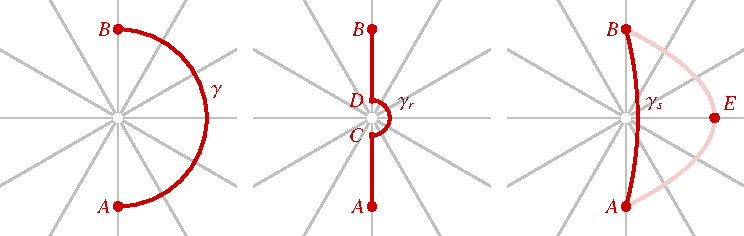
\includegraphics{chapters/030-kurvenintegral/images/wege.pdf}
\caption{Verschiedene Wege zur Berechnung des Integrals der 1-Form
$r\,d\varphi$.
Die Wege, die nahe am Nullpunkt vorbeigehen, ergeben nur sehr kleine
Werte für das Integral, während der Kreisbogen $\gamma$ des
Einheitskreises den Wert $\pi$ ergibt.
\label{buch:kurvenintegral:differential:fig:wege}}
\end{figure}

Wir betrachten das Gebiet $M=\mathbb{R}^2\setminus\{0\}$, also die
Ebene ohne den Nullpunkt.
Statt in $x$-$y$-Koordinaten kann sie auch in Polarkoordinaten
beschrieben werden.
\index{Polarkoordinaten}%
Die Umrechnung ist durch die Abbildung
\[
(x,y) \mapsto (r,\varphi)=\biggl(\sqrt{x^2+y^2},\arctan\frac{y}{x}\biggr)
\]
gegeben.

Auf dem Gebiet $M$ soll jetzt die 1-Form $r\,d\varphi$ betrachtet und
zwischen den beiden Punkten $A=(0,-1)$ und $B=(0,1)$ integriert werden.
In Polarkoordinaten haben die beiden Punkte beide den Radius $r=1$,
aber der Polarwinkel ist $\varphi(A) = -\frac{\pi}2$ und
$\varphi(B)=\frac{\pi}2$.
Als Weg $\gamma$ wird der Abschnitt des Einheitskreises verwendet, der in
Polarkoordinaten durch $[-\frac{\pi}2,\frac{\pi}2]\to M:t\mapsto (1,t)$ 
gegeben ist.
Das Integral von $r\,d\varphi$ ist
\begin{equation}
\int_{\gamma} r\,d\varphi
=
\int_{-\frac{\pi}2}^{\frac{\pi}2}
1\cdot \dot{\varphi}\,dt
=
\int_{-\frac{\pi}2}^{\frac{\pi}2}\,dt
=
\bigl[t\bigr]_{-\frac{\pi}2}^{\frac{\pi}2}
=
\pi.
\label{buch:kurvenintegral:differential:eqn:halbkreis}
\end{equation}
Der Wert ändert sich jedoch, wenn ein anderer Weg gewählt wird.
Der Weg $\gamma_r$ setzt sich zusammen aus einem vertikalen
Segment von $A$ zum Punkt $C$, einem Halbkreisbogen mit
Radius $r$ von $C$ zu $D$ und einem weiteren vertikalen Segment
von $D$ zu $B$.
Da sich der Polarwinkel entlang der geraden Segmente nicht ändert,
verschwindet das Integral von $r\,df$ über die diese Segmente.
Das Integral über den Kreisbogen kann wie in 
\eqref{buch:kurvenintegral:differential:eqn:halbkreis}
berechnet werden, mit dem einzigen Unterschied, dass der Faktor $r$
jetzt nicht $1$ ist.
Das Integral hat daher den Wert $r\pi$ und es folgt
\[
\int_{\gamma_r} r\,d\varphi
=
\underbrace{\int_{AC} r\,d\varphi}_{\displaystyle = 0}
+
\underbrace{\int_{CD} r\,d\varphi}_{\displaystyle = r\pi}
+
\underbrace{\int_{DB} r\,d\varphi}_{\displaystyle = 0}
=
r\pi.
\]
Indem man den Radius $r$ des Kreisbogens klein macht, kann das Integral
also beliebig klein gemacht werden.

Gegen das Argument kann eingewendet werden, dass die verwendete 
Kurve $\gamma_r$ nicht differenzierbar ist.
Die entwickelte Theorie ist daher gar nicht anwendbar.
Man könnte aber auch einen Parabelbogen, der durch die Punkte 
$A$, $E$ und $B$ geht, differenzierbar deformieren.
Der Weg 
\[
\gamma_s
\colon
[-1,1]
\to
\mathbb{R}^2
:
t\mapsto (s(1-t)(1+t), t)=(s(1-t^2),t)
\]
geht durch die Punkte $A$, $B$ und $(s,0)$ in kartesischen
Koordinaten.
Insbesondere geht er im Abstand $s$ am Nullpunkt vorbei.
Da $\gamma_s$ in kartesischen Koordinaten gegeben ist, muss
dazu die 1-Form $r\,d\varphi$ erst in die $x$-$y$-Karte umgerechnet
werden.

Das Differential $d\varphi$ in $x$-$y$-Koordinaten ist
\begin{align*}
d\varphi
&=
d\arctan\frac{y}{x}
=
\frac{\partial}{\partial x}\arctan\frac{y}{x}\,dx
+
\frac{\partial}{\partial y}\arctan\frac{y}{x}\,dy
\\
&=
-\frac{y}{x^2+y^2}\,dx
+
\frac{x}{x^2+y^2}\,dy
=
-\frac{y}{r^2}\,dx
+
\frac{x}{r^2}\,dy
\end{align*}
Die 1-Form
\[
r\,d\varphi
=
-\frac{y}{\sqrt{x^2+y^2}}\,dx
+
\frac{x}{\sqrt{x^2+y^2}}\,dy
=
-\frac{y}{r}\,dx
+
\frac{x}{r}\,dy
\]
ist damit in $x$-$y$-Koordinaten ausgedrückt.

Für die Berechnung des Integrals entlang des Weges $\gamma_s$ werden
die Ableitungen der Koordinaten nach dem Parameter $t$ benötigt, sie
sind
\begin{align*}
\dot{x}(t) &= \frac{d}{dt} s(1-t^2) = -2st \\
\dot{y}(t) &= \frac{d}{dt} t = 1.
\end{align*}
Das Integral entlang des Weges $\gamma_s$ muss jetzt als das Integral
\begin{align*}
\int_{\gamma_s} r\,d\varphi
&=
\int_{-1}^1
-\frac{t}{\sqrt{s^2(1-t^2)^2+1}} \dot{x}(t)
+\frac{s(1-t^2)}{\sqrt{(1-t^2)^2+1}} \dot{y}(t)
\,dt
\\
&=
\int_{-1}^1
\frac{2st^2}{\sqrt{s^2(1-t^2)^2+1}} 
+\frac{s(1-t^2)}{\sqrt{s^2(1-t^2)^2+1}}
\,dt
\\
&=
s\int_{-1}^1
\frac{2t^2+1-t^2}{\sqrt{s^2(1-t^2)^2+1}}
\,dt
\end{align*}
Im Integranden
\[
f(t,s)
=
\frac{s(t^2+1)}{\sqrt{s^2(1-t^2)^2+1}}
\]
nimmt der Zähler das Maximum in den Intervallenden bei $\pm 1$ an.
Der Nenner hat dort sein Minimum.
Daher ist das Maximum des Integranden bei $t=\pm1$, wo der Funktionswert
$2s$ ist.
Das Integral kann damit nach oben durch den grössten
Wert des Integranden als
\[
\int_{\gamma_s} r\,d\varphi
=
\int_{-1}^1 f(t,s)\,dt
=
2 \max_{t\in[-1,1]} f(t,s)
=
4s
\]
abgeschätzt werden.
Je kleiner $s$ wird, desto kleiner wird daher auch das Wegintegral.
Dies zeigt erneut, dass durch einen Weg, der nahe am Nullpunkt vorbeiführt,
das Wegintegral beliebig klein gemacht werden kann und insbesondere
sehr stark von der Wahl des Weges abhängig ist.
\end{beispiel}

%
% Richtungsableitung
%
\subsection{Richtungsableitung}
Die Richtungsableitung einer Funktion 
\index{Richtungsableitung}%
\[
f\colon
\mathbb{R}^n\to\mathbb{R}
:
(x^1,\dots,x^n)\mapsto f(x^1,\dots,x^n)
\]
von $n$ Variablen an der Stelle $x\in\mathbb{R}^n$ in Richtung
eines Vektors $\vec{v}\in\mathbb{R}^n$ ist gegeben durch
\begin{align}
D_{\vec{v}}f(x)
&=
\frac{d}{dt}
f(x+t\vec{v})
\bigg|_{t=0}
=
\frac{d}{dt}
f(x^1+tv^1,\dots,x^n+tv^n)\bigg|_{t=0}
\notag
\\
&=
\frac{\partial f}{\partial x^1}(x)v^1
+
\dots
+
\frac{\partial f}{\partial x^n}(x)v^n
=
\frac{\partial f}{\partial x^i}(x)\,v^i
\label{buch:kurvenintegral:differential:eqn:ricthungsableitung}
\end{align}
(man beachte die Summationskonvention).
Die Richtungsableitung ist also nur ein Spezialfall der Ableitung
einer Funktion entlang einer Kurve für eine speziell gewählte
Kurve.
In der Karte mit den $x^i$-Koordinaten ist die Kurve nämlich die Gerade
\[
x^i(t) = x^i(0) + tv^i
\]
mit dem Richtungsvektor mit Komponenten $v^i$.
\index{Richtungsvektor}%

Insbesondere kann man die Richtungsableitung mit dem Differential
als
\[
D_{\vec{v}}f(x)
=
\langle
df(x),
V
\rangle
\]
schreiben, wobei $V$ der Tangentialvektor ist, der in der Karte
der $x^i$-Koordinaten die Komponenten $v^i$ hat.
Das Differential $df$ verallgemeinert also die Idee der 
Richtungsableitung aof beliebige Koordinantensysteme.


%
% Gradient
%
\subsection{Gradient}
In der klassischen Vektoranalysis schreibt man den Ausdruck
\eqref{buch:kurvenintegral:differential:eqn:ricthungsableitung}
für die Richtungsableitung als Skalarprodukt
\[
D_{\vec{v}}f(x)
=
\renewcommand{\arraystretch}{1.5}
\begin{pmatrix}
\displaystyle
\frac{\partial f}{\partial x^1}(x)\\
\vdots\\
\displaystyle
\frac{\partial f}{\partial x^n}(x)
\end{pmatrix}
\cdot
\vec{v}
\]
und nennt den Vektor
\[
\renewcommand{\arraystretch}{1.5}
\begin{pmatrix}
\displaystyle
\frac{\partial f}{\partial x^1}(x)\\
\vdots\\
\displaystyle
\frac{\partial f}{\partial x^n}(x)
\end{pmatrix}
=
\operatorname{grad}f(x)
=
\nabla f(x)
\]
der partiellen Ableitungen von $f$ nach den
Variablen auch den {\em Gradienten}
\index{Gradient}%
der Funktion $f$.
Der Operator $\nabla$ heisst auch der Nabla-Operator\footnote{Das Zeichen
$\nabla$ wurde von William Rowan Hamilton in der Quaternionenanalysis
\index{Nabla-Operator}%
\index{nabla@$\nabla$}%
als auf den Kopf gestelltes $\Delta$ eingeführt.
Der Theologe William Robertson Smith nannte es Nabla, weil
\index{Smith, William Robertson}%
es ihn an die Form eines so genannten Saiteninstruments aus dem
alten Israel erinnerte.}.

Unter allen Richtungsvektoren $\vec{v}$ mit Länge $1$ wird die
Richtungsableitung
\[
D_{\vec{v}}f(x)
=
\operatorname{grad}f(x)\cdot \vec{v}
=
|\operatorname{grad}f(x)|\;|\vec{v}|\;\cos\alpha
\]
genau dann maximal, wenn der Zwischenwinkel $\alpha$ zwischen
dem Gradienten $\operatorname{grad}f(x)$ und der Richtung $\vec{v}$
verschwindet.
Der Gradient zeigt daher in die Richtung, in der die Funktion am
schnellsten zunimmt.

%
% Der inverse metrische Tensor
%
\subsubsection{Der inverse metrische Tensor}
Die Interpretation des Wertes der 1-Form $df$ auf dem Tangentialvektor $V$ 
als Skalarprodukt des Gradientenvektors $\nabla f(x)$ mit dem
Richtungsvektor $\vec{v}$ verletzt die Regel, dass die Gesetzmässigkeiten
unabhängig von den Koordinatensystemen formuliert werden sollen.
Die Interpretation von
\eqref{buch:kurvenintegral:differential:eqn:ricthungsableitung}
als Skalarprodukt nimmt an, dass an der Stelle $x$ die Koordinatenrichtungen
orthonormiert sind.
Koordinatenunabhängig kann dies nur formuliert werden, wenn ein metrischer
Tensor $g_{ik}$ zur Verfügung steht.
Dann kann man nach einem Vektor $r$ mit den Komponenten $r^k$ fragen,
der über die Formel
\[
\langle df(x),v\rangle
=
\frac{\partial f}{\partial x^i}(x)\,v^i
=
g_{ik} r^k\,v^i
\]
die Richtungsableitung reproduziert.
Da dies für jeden Vektor $v^i$ gilt, muss für jedes $i$ die Gleichung
\begin{equation}
g_{ik}r^k = \frac{\partial f}{\partial x^i}(x)
\label{buch:kurvenintegral:differential:eqn:ggleichung}
\end{equation}
gelten.
Dies ist ein lineares Gleichungssystem mit der symmetrischen
Koeffizientenmatrix $g_{ik}$.
Da der metrische Tensor positiv definit ist, gibt es nur einen
Vektor $r^k$, der das Gleichungssystem löst.

Das Gleichungssystem~\eqref{buch:kurvenintegral:differential:eqn:ggleichung}
kann mit der inversen Matrix der Koeffizientenmatrix gelöst
werden.
Ist $G$ die Matrix mit den Einträgen $g_{ik}$, dann schreiben wir
die inverse Matrix $G^{-1}$ von
\index{metrischer Tensor, invers}%
\[
G
=
\begin{pmatrix}
g_{11}&\dots &g_{1n}\\
\vdots&\ddots&\vdots\\
g_{n1}&\dots &g_{nn}
\end{pmatrix}
\qquad
\text{mit den Einträgen}
\qquad
G^{-1}
= 
\begin{pmatrix}
g^{11}&\dots &g^{1n}\\
\vdots&\ddots&\vdots\\
g^{n1}&\dots &g^{nn}
\end{pmatrix}.
\]
Die Matrix $G^{-1}$ ist ebenfalls symmetrisch.
Die Bedingung $G^{-1}G=I$ wird in Komponenten durch
\[
g^{ik}g_{kl}
=
\delta^i\mathstrut_l
\]
ausgedrückt.

Die Lösung des
Gleichungssystems~\eqref{buch:kurvenintegral:differential:eqn:ggleichung}
ist jetzt durch das Produkt $G^{-1}r$ mit den Komponenten
\[
r^k = g^{ki}\frac{\partial f}{\partial x^i}
\]
gegeben.
Die Rolle des Gradienten wird also vom kovarianten Tensor
\[
g^{ki}\frac{\partial f}{\partial x^i}
\]
übernommen.

Für eine orthonormierte Basis ist der metrische Tensor $g_{ik}=\delta_{ik}$
besonderes einfach, die Matrix $G$ ist die Einheitsmatrix und die 
Inverse ist $G^{-1}=I^{-1}$ ist ebenfalls die Einheitsmatrix.
In diesem Fall ist der Gradient also durch
\[
g^{ki}\frac{\partial f}{\partial x^i}(x)
=
\delta^{ki}\frac{\partial f}{\partial x^i}(x)
=
\frac{\partial f}{\partial x^k}(x)
\]
gegeben, die der klassischen Definition des Gradienten entspricht.

%
% Basis für den metrischen Tensor
%
\subsubsection{Basis für den metrischen Tensor}
Der metrische Tensor ist eine Bilinearform.
Hält man ein Argument fest, muss er sich als Linearform schreiben lassen,
deren Koeffizienten als Linearkombination verstanden werden können.
Wir schreiben daher $dx^i\otimes dx^k$ für eine Bilinearform, die auf
\index{o@$\otimes$}%
den Vektoren $\partial/\partial x^i$ und $\partial/\partial x^k$ den
Wert $1$ annimmt, und $0$ auf allen anderen Paaren von Basisvektoren
dieser Form.
Das Zeichen $\otimes$ soll die beiden Argumente der Bilinearform
auseinanderhalten aber dennoch daran erinnern, dass die Funktion
sich bilinear, also wie ein Produkt verhält.

%
% Kontravarianz des inversen metrischen Tensors
%
\subsubsection{Kontravarianz des inversen metrischen Tensors}
Bei einem Koordinatenwechsel vom $(x^1,\dots,x^n)$-Koordinatensystem
mit metrischem Tensor $g_{ik}$ in das $(y^1,\dots,y^n)$-Koordinatensystem
mit dem metrischen Tensor $h_{ik}$ mit den partiellen Ableitungen
der $y$-Koordinaten nach den $x$-Koordinaten umgerechnet.
Aus der Rechnung
\begin{align*}
\sum_{i,k=1}^n
h_{ik} \, dy^i \otimes dy^k
&=
\sum_{i,k=1}^n
h_{ik}
\biggl(\sum_{l=1}^n \frac{\partial y^i}{\partial x^l}\, dx^l \biggr)
\otimes
\biggl(\sum_{m=1}^n \frac{\partial y^k}{\partial x^m}\, dx^m \biggr)
\\
&=
\sum_{l,m=1}^n
\biggl(
\underbrace{
\sum_{i,k=1}^n h_{ik}
\frac{\partial y^i}{\partial x^l}
\frac{\partial y^k}{\partial x^m}
}_{\displaystyle = g_{lm}}
\biggr)
\,
dx^l\otimes dx^m
\end{align*}
folgt daher, dass
\begin{equation}
g_{lm}
=
\sum_{i,k=1}^n h_{ik}
\frac{\partial y^i}{\partial x^l}
\frac{\partial y^k}{\partial x^m}.
\label{buch:kurvenintegral:differential:eqn:gkovarianz}
\end{equation}
Dies ist das erwartete Resultat für einen Tensor mit zwei unteren 
und daher kovarianten Indizes.

Für die metrischen Tensoren $g^{ik}$, die ein Skalarprodukt für
1-Formen definieren, kann eine analoge Rechnung durchgeführt werden.
Dabei wird verwendet, dass
\[
\frac{\partial}{\partial y^i}
=
\sum_{k=1}^n
\frac{\partial x^k}{\partial y^i}
\,
\frac{\partial}{\partial x^k}
\qquad\text{und}\qquad
\frac{\partial}{\partial x^k}
=
\sum_{i=1}^n
\frac{\partial y^i}{\partial x^k}
\,
\frac{\partial}{\partial x^i}.
\]
Eingesetzt in die Transformationsformel für Metrik von Formen folgt
\begin{align*}
\sum_{k,i=1}^n
g^{ik} \frac{\partial}{\partial x^i}\otimes \frac{\partial}{\partial x^k}
&=
\sum_{i,k=1}^n
g^{ik}
\biggl(
\sum_{l=1}^n \frac{\partial y^l}{\partial x^i}\frac{\partial}{\partial y^l}
\biggr)
\otimes
\biggl(
\sum_{m=1}^n \frac{\partial y^m}{\partial x^k}\frac{\partial}{\partial y^m}
\biggr)
\\
&=
\sum_{l,m=1}^n
\biggl(
\sum_{i,k=1}^n
g^{ik}
\frac{\partial y^l}{\partial x^i}
\frac{\partial y^m}{\partial x^k}
\biggr)
\,
\frac{\partial}{\partial y^l}
\otimes
\frac{\partial}{\partial y^m}
\intertext{und daher}
h^{lm}
&=
\sum_{i,k=1}^n
g^{ik}
\frac{\partial y^l}{\partial x^i}
\frac{\partial y^m}{\partial x^k}.
\end{align*}
Die Transformation erfolgt also im Gegensatz zu den Komponenten
$g_{ik}$ in der umgekehrten Richtung, was zeigt, dass die $g^{ik}$
kontravariant sind.

%
% Indizes anheben und absenken
%
\subsubsection{Indizes anheben und absenken}
Der Tensor $g_{ik}$ hat schon in
Abschnitt~\ref{buch:kurvenintegral:1formen:subsection:linearformen}
ermöglicht, aus einem Vektor, also einem kontravarianten Tensor erster
Stufe, eine Linearform, also einen kovarianten Tensor zu machen.
Mit dem Tensor $g^{ik}$ gelingt es jetzt auch, aus einem kontravarianten
Index einen kovarianten zu machen.
Diese Operationen sind auf jeden beliebigen Index eines Tensors
anwendbar.

\begin{definition}[Anheben und Absenken von Indizes]
\label{buch:kurvenintegral:differential:def:musikalisch}
Ein kontravarianter Index $i$ eines Tensors $A^i$ wird durch
$g_{ki}A^i$ zu einem kovarianten Index $k$ {\em abgesenkt}.
\index{absenken, Index}%
Ein kovarianter Index $i$ eines Tensors $B_i$ wird durch
$g^{il}B_i$ zu einem kontravarianten Index {\em angehoben}.
\index{anheben, Index}%
\end{definition}

Die Operationen des Anhebens und Absenkens von Indizes mithilfe
des metrischen Tensors bzw.~der seiner Inversen werden manchmal
als $A\mapsto A^\flat$ für das Absenken und $B\mapsto B^\sharp$
für das anheben notiert.
Sie werden auch die musikalischen Operationen genannt, da
in der musikalischen Notenschrift das Zeichen $\sharp$ die
Anhebung einer Note um einen halben Ton bedeutet, während
$\flat$ die Absenkung einer Note um eine halben Ton bedeutet.

%
% Konforme Abbildungen
%
\subsubsection{Konforme Abbildungen}
Eine Abbildung heisst {\em konform}, wenn Sie winkeltreu ist.
Die Länge von Vektoren darf also ändern, nicht aber der Winkel.
Da Winkel mit der Skalarproduktformel
\[
\cos \angle(X,Y)
=
\frac{
\langle X,Y \rangle
}{
\!\sqrt{\langle X, X\rangle}\cdot\!\sqrt{\langle Y,Y\rangle}
}
\]
berechnet werden können, darf sich das Skalarprodukt unter einer
konformen Abbildung nur um einen gemeinsamen Faktor ändern.
Mit der Notation von
\eqref{buch:kurvenintegral:differential:eqn:gkovarianz}
folgt daher, dass
\[
g_{ik} = s\,h_{ik}
\quad\Rightarrow\quad
g_{ik}
=
\sum_{l,m=1}^n
\frac{\partial y^l}{\partial x^i}
\frac{\partial y^m}{\partial x^k}
g_{lm}
\]
als Bedingung dafür, dass die Koordinatenwechselabbildung
konform ist.

\begin{beispiel}
Die stereographische Projektion von Beispiel 
\ref{buch:koordinaten:diffmannig:beispiel:stereographisch}
ist konform, wie mit einer direkten, aber im Übrigen nicht
besonders interessanten Rechnung nachgewiesen werden kann.
\end{beispiel}

%
% Die Mercator-Projektion
%
\subsubsection{Die Mercator-Projektion}
Die sogenannte Mercator-Projektion bildet Punkte $(\vartheta,\beta)$
\index{Mercator-Projektion}%
auf der Oberfläche der Einheitskugel auf einen Zylinder mit Koordinaten
$(\varphi,z)$ ab, der die Kugel im Äquator berührt.
\index{Einheitskugel}%
Wir verwenden die vom Äquator gemessene geographische Breite $\beta$
\index{Aquator@Äquator}%
anstelle des bei Kugelkoordinaten üblichen Polabstandes $\vartheta$.
Sie ist aber nicht eine geometrische Zentralprojektion, vielmehr wird die
$z$-Koordinate durch eine nichtlineare Funktion $z(\beta)$
gegeben.

Zunächst muss der metrische Tensor für die Kugeloberfläche
berechnet werden.
Die Kugelkoordinaten sind orthogonal, der metrische Tensor wird
eine Diagonalmatrix, genauer
\[
g
=
\begin{pmatrix}
 1 & 0           \\
 0 & \cos^2\beta
\end{pmatrix}.
\]
Da der Zylinder nur eine ``aufgerollte Ebene'' ist, ist die Metrik
auf dem Zylinder durch die Einheitsmatrix
\[
h = \begin{pmatrix} 1&0\\0&1\end{pmatrix}
\]
gegeben.

Die Koordinatentransformation ist
\[
S^2\to\mathbb{R}^2
:
(\varphi,\beta) \mapsto (\varphi, z(\beta)).
\]
Die zugehörige Jacobimatrix ist
\[
J
=
\frac{\partial(\varphi,z)}{\partial(\varphi,\beta)}
=
\begin{pmatrix}
 1 & 0 \\
 0 & f'(\beta)
\end{pmatrix}.
\]
Transformiert man $g$ mit dieser Matrix, muss ein Vielfaches der
Einheitsmatrix entstehen.
Die Transformation liefert
\begin{align*}
J^tgJ
&=
\begin{pmatrix}
 1 & 0 \\
 0 & f'(\beta)
\end{pmatrix}
\begin{pmatrix}
 1 & 0           \\
 0 & \cos^2\beta
\end{pmatrix}
\begin{pmatrix}
 1 & 0 \\
 0 & f'(\beta)
\end{pmatrix}
\\
&=
\begin{pmatrix}
1&0\\
0&f'(\beta)^2\cos^2\beta
\end{pmatrix}
=
I
\qquad\Rightarrow\qquad
f'(\beta)^2\cos^2\beta = 1.
\end{align*}
Daraus ergibt sich die Differentialgleichung
\[
f'(\beta)=\frac{1}{\cos \beta}
\qquad\text{mit der Anfangsbedingung}\qquad
f(0)=0.
\]
Sie kann durch Integration gelöst werden, die Lösung ist
\[
f(\beta)
=
\int_0^\beta \frac{dt}{\cos t}
=
\frac12 \log\biggl(
\frac{1+\sin\beta}{1-\sin\beta}
\biggr).
\]
Die Mercator-Projektion ist daher gegeben durch
\begin{equation}
(\varphi,\beta) \mapsto \biggl(
\varphi,\frac12\log\biggl(\frac{1+\sin\beta}{1-\sin\beta}\biggr)
\biggr).
\label{buch:kurvenintegral:differential:eqn:mercatorprojektion}
\end{equation}
%
% fig-mercator.tex
%
% (c) 2025 Prof Dr Andreas Müller
%
\begin{figure}
\centering
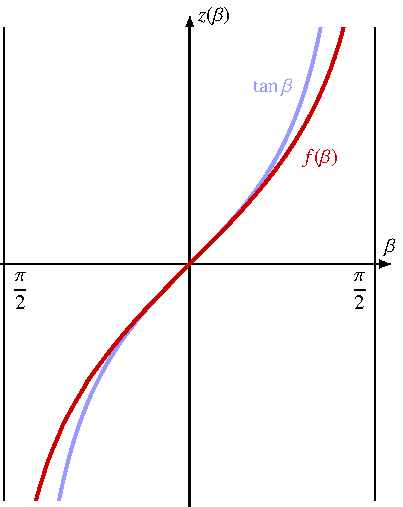
\includegraphics{chapters/030-kurvenintegral/images/mercator.pdf}
\caption{Die Funktion $f(\beta)$, die die Mercator-Projektion definiert,
dargestellt als die {\color{darkred}rote} Kurve.
Zum Vergleich ist auch die Funktion $\tan\beta$ dargestellt, die zur
Zentralprojektion auf den Zylinder führt.
\label{buch:kurvenintegral:fig:mercator}}
\end{figure}
%
Die Funktion $f(\beta)$ ist auch in
Abbildung~\ref{buch:kurvenintegral:fig:mercator} dargestellt.
 
%
% Differentialgleichungen
%
\subsection{Differentialgleichungen}
Eine $1$-Form $\alpha = \alpha_i\,dx^i$ auf einer zweidimensionalen
Mannigfaltigkeit ist in jedem Punkt der Mannigfaltigkeit eine lineare
Funktion, die einem Tangentialvektor einen Zahlenwert zuordnet.
Falls die Linearform nicht verschwindet, kann sie nur Rang $1$
haben.
Es gibt daher einen eindimensionalen Unterraum von Vektoren $X$, die
von der $1$-Form zu $0$ gemacht werden.

Ein Tangentialvektor kann durch eine parametrisierte Kurve repräsentiert
werden.
In Koordinaten sind die Komponenten des Tangentialvektors durch
die Ableitungen der $\dot{x}^i$ gegeben.
Ein Tangentialvektor, der die 1-Form zum Verschwinden bringt, erfüllt
daher
\begin{align*}
0
&=
\langle\alpha, X\rangle
=
\langle
\alpha_i\,dx^i,
X
\rangle
\\
&=
\biggl\langle
\alpha_i(x(t))\,dx^i,
\dot{x}^k(t)\frac{\partial}{\partial x^k}
\biggr\rangle
\\
&=
\sum_{i=1}^n
\alpha_i(x(t))
\biggl\langle
dx^i,\frac{\partial}{\partial x^k}
\biggr\rangle
\dot{x}^k(t)
=
\alpha_i(x(t))\delta_{ik}\dot{x}^k(t)
\\
&=
\alpha_i(x(t))\dot{x}^i(t).
\end{align*}

In zwei Dimensionen lässt sich das noch etwas weiter treiben.
Falls $\alpha_2(x(t))\ne 0$ ist, kann die Gleichung
\begin{equation}
\alpha_1(x(t))\, \dot{x}^1(t) + \alpha_2(x(t))\,\dot{x}^2(t) = 0
\label{buch:kurvenintegral:differential:eqn:1formsteigung}
\end{equation}
nach
\[
\frac{\dot{x}^2(t)}{\dot{x}^1(t)}
=
\frac{\alpha_1(x(t))}{\alpha_2(x(t))}
\]
aufgelöst werden.
Dies ist die Steigung der Kurve in einem 
$(x^1,x^2)$-Koordinatensystem.
Falls $\alpha_2(x(t))=0$ folgt aus
\eqref{buch:kurvenintegral:differential:eqn:1formsteigung}, dass
$\dot{x}^1(t)=0$ sein muss, dass die Kurve also eine Tangentenrichtung
parallel zur $x^2$-Richtung hat.

Die Gleichung $\langle\alpha,X\rangle=0$ legt daher die Richtung
einer Lösungskurve vor.
Eine 1-Form definiert somit ein Richtungsfeld auf einer zweidimensionalen
Mannigfaltigkeit genauso wie eine gewöhnliche Differentialgleichung
der Form $y'=f(x,y)$ ein Richtungsfeld auf der $x$-$y$-Ebene festlegt.

%
% Separation der Variablen
%
\subsubsection{Separation der Variablen}
Wenn die Koeffizienten $\alpha_i(x)$ der 1-Form nur von jeweils der einen
Variable $x^i$ abhängen, dann kann man die beiden 1-Formen
$\alpha_1\,dx^1$ und $\alpha_2\,dx^2$ entlang der Lösungskurve
integrieren, man kann also schreiben
\begin{align}
\alpha_1(x^1)\,dx^1
+
\alpha_2(x^2)\,dx^2
&=0
&&\Rightarrow&
\alpha_1(x^1)\,dx^1
&=
-
\alpha_2(x^2)\,dx^2
\notag
\\
&
&&\Rightarrow&
\int \alpha_1(x^1)\,dx^1
&=
-\int \alpha_2(x^2)\,dx^2.
\label{buch:kurvenintegral:differential:eqn:separation}
\end{align}
Da in $\alpha_1$ nur die Variable $x^1$ vorkommt und in $\alpha_2$
nur die Variable $x^2$, lassen sich die beiden Integrale auf den
beiden Seiten \eqref{buch:kurvenintegral:differential:eqn:separation}
als gewöhnliche Integrale ausführen und liefern eine Gleichung,
die $x^1$ und $x^2$ erfüllen müssen.
Diese kann man jetzt nach $x^2$ auflösen und damit eine Lösung der
Differentialgleichung in der Form einer Funktion $x^2(x^1)$ finden.

Die eben beschriebene Vorgehensweise erinnert nicht nur oberflächlich
an die Methode der Separation der Variablen, die man in einer
Anfängervorlesung über gewöhnliche Differentialgleichung typischerweise
kennenlernt.
In der Theorie der Ableitung und des Riemann-Integrals sind die Zeichen
$dx^1$ und $dx^2$ nur Symbole, die für sich allein keine
wohldefinierte mathematische Bedeutung haben.
Die Vorgehensweise in der Methode der Separation der Variablen ist
daher nur formal und nur dadurch gerechtfertigt, dass es am Schluss
``aufgeht''.
Die Theorie der 1-Formen und der Integration von 1-Formen zeigt,
wie diese Lösungsmethode mathematisch widerspruchsfrei formuliert
werden kann.

%
% Die Differentialgleichung der Loxodrome
%
\subsubsection{Die Differentialgleichung der Loxodrome}
Die Loxodrome auf der Kugeloberfläche wird in einer Mercator-Projektion
zu einer Geraden.
Betrachten wir die Mercator-Projektion als Karte der Kugeloberfläche
mit den Koordinaten $(\varphi,z)$, dann erfüllen die Geraden mit
Steigung $k$ in Parameterdarstellung die Gleichung
\[
\frac{\dot{z}(t)}{\dot{\varphi}(t)}
=
k.
\]
Die Differentialgleichung kann man als $1$-Form 
\begin{equation}
\alpha
=
k\,d\varphi - dz
\label{buch:kurvenintegral:differential:mercatorform}
\end{equation}
schreiben.

Die Mercator-Projektion ist in geographischen Koordinaten
auf der Kugelaberfläche die Abbildung
\[
f\colon
\mathbb{R}^2\to\mathbb{R}^2
:
(\varphi,\beta)
\mapsto
(\varphi,z)
=
(\varphi,f(\beta))
=
\biggl(\varphi,\frac12\log\frac{1+\sin\beta}{1-\sin\beta}\biggr).
\]
Durch Transport der 1-Form
\eqref{buch:kurvenintegral:differential:mercatorform}
mithilfe der Mercator-Projektion
von~\eqref{buch:kurvenintegral:differential:eqn:mercatorprojektion}
bekommt man aus
\begin{equation}
dz
=
f'(\beta)\,d\beta
=
\frac{1}{\cos\beta}\,d\beta
\qquad\Rightarrow\qquad
\alpha
=
k\,d\varphi-\frac{1}{\cos\beta}\,d\beta
\label{buch:kurvenintegral:differential:mercatorsepariert}
\end{equation}

Wir suchen eine Lösung der Differentialgleichung $\alpha=0$
als Funktion $\vartheta(\varphi)$.
Die $1$-Form
\eqref{buch:kurvenintegral:differential:mercatorsepariert}
hat die Eigenschaft, dass die Koeffizienten nur von jeweils
einer Variablen abhängen.
Somit sind die Voraussetzungen für die Anwendung der Methode
der Separation der Variablen gegeben.
Die Differentialgleichung kann damit durch Integration
\[
k\,d\varphi=\frac{1}{\cos\beta}\,d\beta
\quad
\Rightarrow
\quad
k\int d\varphi
=-
\int \frac{d\beta}{\cos\beta}
\quad
\Rightarrow
\quad
k\varphi + C
=
\frac12
\log\frac{1+\sin\beta}{1-\sin\beta}
\]
gelöst werden.
Die Funktion auf der rechten Seite ist auch der $\operatorname{artanh}$
von $\sin\beta$, daher kann man die Lösung für die Loxodrome auch
als
\[
\sin\beta
=
\tanh(k\varphi+C)
\quad
\Rightarrow
\quad
\beta = \arcsin\tanh(k\varphi+C)
\]
schreiben.

